\documentclass[twoside]{book}

% Packages required by doxygen
\usepackage{fixltx2e}
\usepackage{calc}
\usepackage{doxygen}
\usepackage[export]{adjustbox} % also loads graphicx
\usepackage{graphicx}
\usepackage[utf8]{inputenc}
\usepackage{makeidx}
\usepackage{multicol}
\usepackage{multirow}
\PassOptionsToPackage{warn}{textcomp}
\usepackage{textcomp}
\usepackage[nointegrals]{wasysym}
\usepackage[table]{xcolor}

% Font selection
\usepackage[T1]{fontenc}
\usepackage[scaled=.90]{helvet}
\usepackage{courier}
\usepackage{amssymb}
\usepackage{sectsty}
\renewcommand{\familydefault}{\sfdefault}
\allsectionsfont{%
  \fontseries{bc}\selectfont%
  \color{darkgray}%
}
\renewcommand{\DoxyLabelFont}{%
  \fontseries{bc}\selectfont%
  \color{darkgray}%
}
\newcommand{\+}{\discretionary{\mbox{\scriptsize$\hookleftarrow$}}{}{}}

% Page & text layout
\usepackage{geometry}
\geometry{%
  a4paper,%
  top=2.5cm,%
  bottom=2.5cm,%
  left=2.5cm,%
  right=2.5cm%
}
\tolerance=750
\hfuzz=15pt
\hbadness=750
\setlength{\emergencystretch}{15pt}
\setlength{\parindent}{0cm}
\setlength{\parskip}{3ex plus 2ex minus 2ex}
\makeatletter
\renewcommand{\paragraph}{%
  \@startsection{paragraph}{4}{0ex}{-1.0ex}{1.0ex}{%
    \normalfont\normalsize\bfseries\SS@parafont%
  }%
}
\renewcommand{\subparagraph}{%
  \@startsection{subparagraph}{5}{0ex}{-1.0ex}{1.0ex}{%
    \normalfont\normalsize\bfseries\SS@subparafont%
  }%
}
\makeatother

% Headers & footers
\usepackage{fancyhdr}
\pagestyle{fancyplain}
\fancyhead[LE]{\fancyplain{}{\bfseries\thepage}}
\fancyhead[CE]{\fancyplain{}{}}
\fancyhead[RE]{\fancyplain{}{\bfseries\leftmark}}
\fancyhead[LO]{\fancyplain{}{\bfseries\rightmark}}
\fancyhead[CO]{\fancyplain{}{}}
\fancyhead[RO]{\fancyplain{}{\bfseries\thepage}}
\fancyfoot[LE]{\fancyplain{}{}}
\fancyfoot[CE]{\fancyplain{}{}}
\fancyfoot[RE]{\fancyplain{}{\bfseries\scriptsize Generated by Doxygen }}
\fancyfoot[LO]{\fancyplain{}{\bfseries\scriptsize Generated by Doxygen }}
\fancyfoot[CO]{\fancyplain{}{}}
\fancyfoot[RO]{\fancyplain{}{}}
\renewcommand{\footrulewidth}{0.4pt}
\renewcommand{\chaptermark}[1]{%
  \markboth{#1}{}%
}
\renewcommand{\sectionmark}[1]{%
  \markright{\thesection\ #1}%
}

% Indices & bibliography
\usepackage{natbib}
\usepackage[titles]{tocloft}
\setcounter{tocdepth}{3}
\setcounter{secnumdepth}{5}
\makeindex

% Hyperlinks (required, but should be loaded last)
\usepackage{ifpdf}
\ifpdf
  \usepackage[pdftex,pagebackref=true]{hyperref}
\else
  \usepackage[ps2pdf,pagebackref=true]{hyperref}
\fi
\hypersetup{%
  colorlinks=true,%
  linkcolor=blue,%
  citecolor=blue,%
  unicode%
}

% Custom commands
\newcommand{\clearemptydoublepage}{%
  \newpage{\pagestyle{empty}\cleardoublepage}%
}

\usepackage{caption}
\captionsetup{labelsep=space,justification=centering,font={bf},singlelinecheck=off,skip=4pt,position=top}

%===== C O N T E N T S =====

\begin{document}

% Titlepage & ToC
\hypersetup{pageanchor=false,
             bookmarksnumbered=true,
             pdfencoding=unicode
            }
\pagenumbering{alph}
\begin{titlepage}
\vspace*{7cm}
\begin{center}%
{\Large Pacman Client \\[1ex]\large v4 }\\
\vspace*{1cm}
{\large Generated by Doxygen 1.8.14}\\
\end{center}
\end{titlepage}
\clearemptydoublepage
\pagenumbering{roman}
\tableofcontents
\clearemptydoublepage
\pagenumbering{arabic}
\hypersetup{pageanchor=true}

%--- Begin generated contents ---
\chapter{Hierarchical Index}
\section{Class Hierarchy}
This inheritance list is sorted roughly, but not completely, alphabetically\+:\begin{DoxyCompactList}
\item \contentsline{section}{Food\+Ball}{\pageref{class_food_ball}}{}
\item \contentsline{section}{Ghost}{\pageref{class_ghost}}{}
\item \contentsline{section}{Map}{\pageref{class_map}}{}
\item \contentsline{section}{Pacman}{\pageref{class_pacman}}{}
\item \contentsline{section}{Power\+Ball}{\pageref{class_power_ball}}{}
\item Q\+Object\begin{DoxyCompactList}
\item \contentsline{section}{Pacman\+Server}{\pageref{class_pacman_server}}{}
\end{DoxyCompactList}
\end{DoxyCompactList}

\chapter{Class Index}
\section{Class List}
Here are the classes, structs, unions and interfaces with brief descriptions\+:\begin{DoxyCompactList}
\item\contentsline{section}{\mbox{\hyperlink{class_ask_for_i_p___interface}{Ask\+For\+I\+P\+\_\+\+Interface}} }{\pageref{class_ask_for_i_p___interface}}{}
\item\contentsline{section}{\mbox{\hyperlink{class_client_connection}{Client\+Connection}} }{\pageref{class_client_connection}}{}
\item\contentsline{section}{\mbox{\hyperlink{class_food_ball}{Food\+Ball}} }{\pageref{class_food_ball}}{}
\item\contentsline{section}{\mbox{\hyperlink{class_game__window}{Game\+\_\+window}} }{\pageref{class_game__window}}{}
\item\contentsline{section}{\mbox{\hyperlink{class_ghost}{Ghost}} }{\pageref{class_ghost}}{}
\item\contentsline{section}{\mbox{\hyperlink{class_map}{Map}} }{\pageref{class_map}}{}
\item\contentsline{section}{\mbox{\hyperlink{class_pacman}{Pacman}} }{\pageref{class_pacman}}{}
\item\contentsline{section}{\mbox{\hyperlink{class_power_ball}{Power\+Ball}} }{\pageref{class_power_ball}}{}
\item\contentsline{section}{\mbox{\hyperlink{class_sounds}{Sounds}} }{\pageref{class_sounds}}{}
\item\contentsline{section}{\mbox{\hyperlink{class_text_screen_message}{Text\+Screen\+Message}} }{\pageref{class_text_screen_message}}{}
\end{DoxyCompactList}

\chapter{Class Documentation}
\hypertarget{class_ask_for_i_p___interface}{}\section{Ask\+For\+I\+P\+\_\+\+Interface Class Reference}
\label{class_ask_for_i_p___interface}\index{Ask\+For\+I\+P\+\_\+\+Interface@{Ask\+For\+I\+P\+\_\+\+Interface}}


{\ttfamily \#include $<$askforipinterface.\+h$>$}

Inheritance diagram for Ask\+For\+I\+P\+\_\+\+Interface\+:\begin{figure}[H]
\begin{center}
\leavevmode
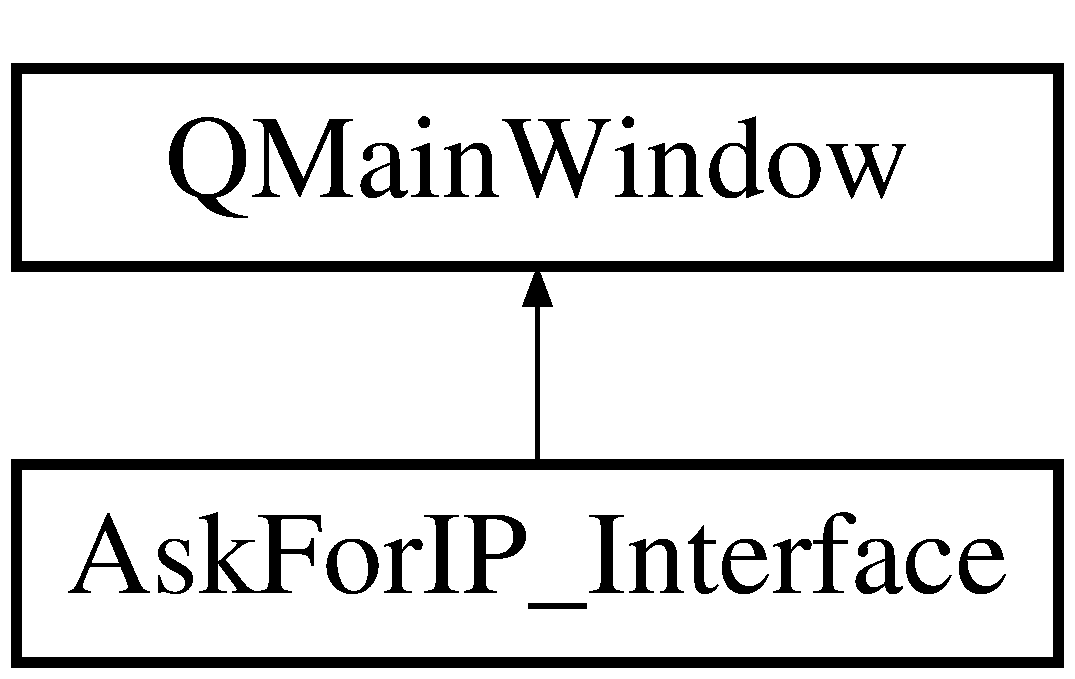
\includegraphics[height=2.000000cm]{class_ask_for_i_p___interface}
\end{center}
\end{figure}
\subsection*{Public Member Functions}
\begin{DoxyCompactItemize}
\item 
\mbox{\hyperlink{class_ask_for_i_p___interface_a76694e9589d8a7a339127e427dd404df}{Ask\+For\+I\+P\+\_\+\+Interface}} (Q\+Widget $\ast$parent=0)
\item 
Q\+Host\+Address \mbox{\hyperlink{class_ask_for_i_p___interface_a825a41d9af858b34f2acdb187ef3c327}{get\+IP}} ()
\item 
uint \mbox{\hyperlink{class_ask_for_i_p___interface_af3d49951f070582d72c125b631f8212d}{get\+Port}} ()
\end{DoxyCompactItemize}


\subsection{Detailed Description}
Class responsible for displaying user interface asking for IP address and port number to connect to 

\subsection{Constructor \& Destructor Documentation}
\mbox{\Hypertarget{class_ask_for_i_p___interface_a76694e9589d8a7a339127e427dd404df}\label{class_ask_for_i_p___interface_a76694e9589d8a7a339127e427dd404df}} 
\index{Ask\+For\+I\+P\+\_\+\+Interface@{Ask\+For\+I\+P\+\_\+\+Interface}!Ask\+For\+I\+P\+\_\+\+Interface@{Ask\+For\+I\+P\+\_\+\+Interface}}
\index{Ask\+For\+I\+P\+\_\+\+Interface@{Ask\+For\+I\+P\+\_\+\+Interface}!Ask\+For\+I\+P\+\_\+\+Interface@{Ask\+For\+I\+P\+\_\+\+Interface}}
\subsubsection{\texorpdfstring{Ask\+For\+I\+P\+\_\+\+Interface()}{AskForIP\_Interface()}}
{\footnotesize\ttfamily Ask\+For\+I\+P\+\_\+\+Interface\+::\+Ask\+For\+I\+P\+\_\+\+Interface (\begin{DoxyParamCaption}\item[{Q\+Widget $\ast$}]{parent = {\ttfamily 0} }\end{DoxyParamCaption})\hspace{0.3cm}{\ttfamily [explicit]}}

Initialize member variables and disable Connect push button 

\subsection{Member Function Documentation}
\mbox{\Hypertarget{class_ask_for_i_p___interface_a825a41d9af858b34f2acdb187ef3c327}\label{class_ask_for_i_p___interface_a825a41d9af858b34f2acdb187ef3c327}} 
\index{Ask\+For\+I\+P\+\_\+\+Interface@{Ask\+For\+I\+P\+\_\+\+Interface}!get\+IP@{get\+IP}}
\index{get\+IP@{get\+IP}!Ask\+For\+I\+P\+\_\+\+Interface@{Ask\+For\+I\+P\+\_\+\+Interface}}
\subsubsection{\texorpdfstring{get\+I\+P()}{getIP()}}
{\footnotesize\ttfamily Q\+Host\+Address Ask\+For\+I\+P\+\_\+\+Interface\+::get\+IP (\begin{DoxyParamCaption}{ }\end{DoxyParamCaption})\hspace{0.3cm}{\ttfamily [inline]}}

Get IP address in form of Q\+Host\+Address \mbox{\Hypertarget{class_ask_for_i_p___interface_af3d49951f070582d72c125b631f8212d}\label{class_ask_for_i_p___interface_af3d49951f070582d72c125b631f8212d}} 
\index{Ask\+For\+I\+P\+\_\+\+Interface@{Ask\+For\+I\+P\+\_\+\+Interface}!get\+Port@{get\+Port}}
\index{get\+Port@{get\+Port}!Ask\+For\+I\+P\+\_\+\+Interface@{Ask\+For\+I\+P\+\_\+\+Interface}}
\subsubsection{\texorpdfstring{get\+Port()}{getPort()}}
{\footnotesize\ttfamily uint Ask\+For\+I\+P\+\_\+\+Interface\+::get\+Port (\begin{DoxyParamCaption}{ }\end{DoxyParamCaption})\hspace{0.3cm}{\ttfamily [inline]}}

Get port number in form of unsigned integer 

The documentation for this class was generated from the following files\+:\begin{DoxyCompactItemize}
\item 
C\+:/\+Users/\+Adam/\+Documents/\+Pacman\+\_\+\+Multiplayer-\/-\/-\/\+Client-\/\+App/askforipinterface.\+h\item 
C\+:/\+Users/\+Adam/\+Documents/\+Pacman\+\_\+\+Multiplayer-\/-\/-\/\+Client-\/\+App/askforipinterface.\+cpp\end{DoxyCompactItemize}

\hypertarget{class_client_connection}{}\section{Client\+Connection Class Reference}
\label{class_client_connection}\index{Client\+Connection@{Client\+Connection}}
Inheritance diagram for Client\+Connection\+:\begin{figure}[H]
\begin{center}
\leavevmode
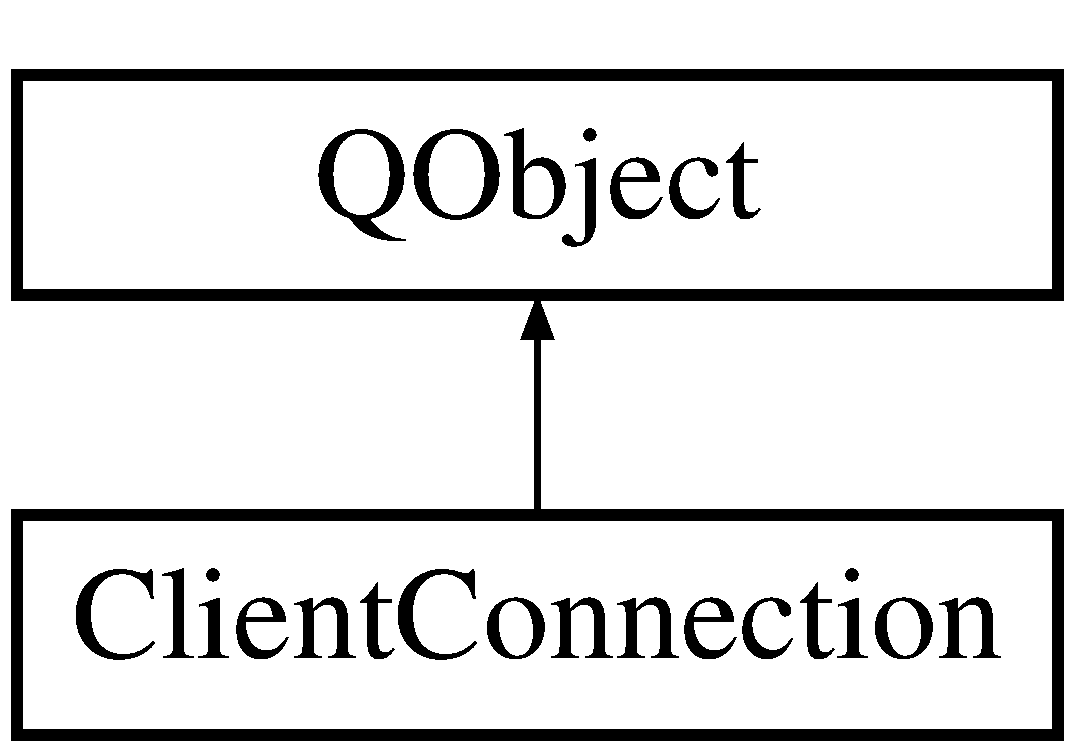
\includegraphics[height=2.000000cm]{class_client_connection}
\end{center}
\end{figure}
\subsection*{Signals}
\begin{DoxyCompactItemize}
\item 
\mbox{\Hypertarget{class_client_connection_a36ede8a48237a964e028c580df771256}\label{class_client_connection_a36ede8a48237a964e028c580df771256}} 
void {\bfseries Game\+Started\+\_\+signal} ()
\end{DoxyCompactItemize}
\subsection*{Public Member Functions}
\begin{DoxyCompactItemize}
\item 
\mbox{\hyperlink{class_client_connection_af7853013395a43befeab1f44b0af863f}{Client\+Connection}} (Q\+Status\+Bar $\ast$\+\_\+statusbar, int $\ast$\+\_\+game\+\_\+state, Q\+Object $\ast$parent=nullptr)
\item 
void \mbox{\hyperlink{class_client_connection_a12d5696ee4d4987e1926d1f8e6626af0}{Request\+Connection}} (Q\+Host\+Address \+\_\+address, uint \+\_\+port)
\item 
void \mbox{\hyperlink{class_client_connection_a2b0ac3043269fc55e415df2c05b880c1}{Send\+Pressed\+Key\+To\+Server}} (char key)
\item 
Q\+Byte\+Array \mbox{\hyperlink{class_client_connection_a24fb529ef10c41be5239afe1928df87e}{get\+Coordinates}} ()
\end{DoxyCompactItemize}


\subsection{Constructor \& Destructor Documentation}
\mbox{\Hypertarget{class_client_connection_af7853013395a43befeab1f44b0af863f}\label{class_client_connection_af7853013395a43befeab1f44b0af863f}} 
\index{Client\+Connection@{Client\+Connection}!Client\+Connection@{Client\+Connection}}
\index{Client\+Connection@{Client\+Connection}!Client\+Connection@{Client\+Connection}}
\subsubsection{\texorpdfstring{Client\+Connection()}{ClientConnection()}}
{\footnotesize\ttfamily Client\+Connection\+::\+Client\+Connection (\begin{DoxyParamCaption}\item[{Q\+Status\+Bar $\ast$}]{\+\_\+statusbar,  }\item[{int $\ast$}]{\+\_\+game\+\_\+state,  }\item[{Q\+Object $\ast$}]{parent = {\ttfamily nullptr} }\end{DoxyParamCaption})\hspace{0.3cm}{\ttfamily [explicit]}}

Initialize member variables, set up client socket and connect its signals and slots 

\subsection{Member Function Documentation}
\mbox{\Hypertarget{class_client_connection_a24fb529ef10c41be5239afe1928df87e}\label{class_client_connection_a24fb529ef10c41be5239afe1928df87e}} 
\index{Client\+Connection@{Client\+Connection}!get\+Coordinates@{get\+Coordinates}}
\index{get\+Coordinates@{get\+Coordinates}!Client\+Connection@{Client\+Connection}}
\subsubsection{\texorpdfstring{get\+Coordinates()}{getCoordinates()}}
{\footnotesize\ttfamily Q\+Byte\+Array Client\+Connection\+::get\+Coordinates (\begin{DoxyParamCaption}{ }\end{DoxyParamCaption})\hspace{0.3cm}{\ttfamily [inline]}}

Get coordinates and data received from server in form of Q\+Byte\+Array \mbox{\Hypertarget{class_client_connection_a12d5696ee4d4987e1926d1f8e6626af0}\label{class_client_connection_a12d5696ee4d4987e1926d1f8e6626af0}} 
\index{Client\+Connection@{Client\+Connection}!Request\+Connection@{Request\+Connection}}
\index{Request\+Connection@{Request\+Connection}!Client\+Connection@{Client\+Connection}}
\subsubsection{\texorpdfstring{Request\+Connection()}{RequestConnection()}}
{\footnotesize\ttfamily void Client\+Connection\+::\+Request\+Connection (\begin{DoxyParamCaption}\item[{Q\+Host\+Address}]{\+\_\+address,  }\item[{uint}]{\+\_\+port }\end{DoxyParamCaption})}

Try to connect with given address and port number \mbox{\Hypertarget{class_client_connection_a2b0ac3043269fc55e415df2c05b880c1}\label{class_client_connection_a2b0ac3043269fc55e415df2c05b880c1}} 
\index{Client\+Connection@{Client\+Connection}!Send\+Pressed\+Key\+To\+Server@{Send\+Pressed\+Key\+To\+Server}}
\index{Send\+Pressed\+Key\+To\+Server@{Send\+Pressed\+Key\+To\+Server}!Client\+Connection@{Client\+Connection}}
\subsubsection{\texorpdfstring{Send\+Pressed\+Key\+To\+Server()}{SendPressedKeyToServer()}}
{\footnotesize\ttfamily void Client\+Connection\+::\+Send\+Pressed\+Key\+To\+Server (\begin{DoxyParamCaption}\item[{char}]{key }\end{DoxyParamCaption})}

Translate pressed key to certain value and send it to server 

The documentation for this class was generated from the following files\+:\begin{DoxyCompactItemize}
\item 
C\+:/\+Users/\+Adam/\+Documents/\+Pacman\+\_\+\+Multiplayer-\/-\/-\/\+Client-\/\+App/clientconnection.\+h\item 
C\+:/\+Users/\+Adam/\+Documents/\+Pacman\+\_\+\+Multiplayer-\/-\/-\/\+Client-\/\+App/clientconnection.\+cpp\end{DoxyCompactItemize}

\hypertarget{class_food_ball}{}\section{Food\+Ball Class Reference}
\label{class_food_ball}\index{Food\+Ball@{Food\+Ball}}
\subsection*{Public Member Functions}
\begin{DoxyCompactItemize}
\item 
\mbox{\hyperlink{class_food_ball_accba761984d128bead135b3864a63ed0}{Food\+Ball}} ()
\item 
Q\+Vector$<$ Q\+Point $>$ \mbox{\hyperlink{class_food_ball_a8426b37d22df239e9f605a4c5fae189a}{get\+Food\+Ball\+Positions}} ()
\end{DoxyCompactItemize}


\subsection{Constructor \& Destructor Documentation}
\mbox{\Hypertarget{class_food_ball_accba761984d128bead135b3864a63ed0}\label{class_food_ball_accba761984d128bead135b3864a63ed0}} 
\index{Food\+Ball@{Food\+Ball}!Food\+Ball@{Food\+Ball}}
\index{Food\+Ball@{Food\+Ball}!Food\+Ball@{Food\+Ball}}
\subsubsection{\texorpdfstring{Food\+Ball()}{FoodBall()}}
{\footnotesize\ttfamily Food\+Ball\+::\+Food\+Ball (\begin{DoxyParamCaption}{ }\end{DoxyParamCaption})}

Initialize member variables and fill foodballpositions vector with Q\+Points representing foodballs coordinates on map 

\subsection{Member Function Documentation}
\mbox{\Hypertarget{class_food_ball_a8426b37d22df239e9f605a4c5fae189a}\label{class_food_ball_a8426b37d22df239e9f605a4c5fae189a}} 
\index{Food\+Ball@{Food\+Ball}!get\+Food\+Ball\+Positions@{get\+Food\+Ball\+Positions}}
\index{get\+Food\+Ball\+Positions@{get\+Food\+Ball\+Positions}!Food\+Ball@{Food\+Ball}}
\subsubsection{\texorpdfstring{get\+Food\+Ball\+Positions()}{getFoodBallPositions()}}
{\footnotesize\ttfamily Q\+Vector$<$Q\+Point$>$ Food\+Ball\+::get\+Food\+Ball\+Positions (\begin{DoxyParamCaption}{ }\end{DoxyParamCaption})\hspace{0.3cm}{\ttfamily [inline]}}

Get generated foodballpositions vector in form of Q\+Vector$<$\+Q\+Point$>$ 

The documentation for this class was generated from the following files\+:\begin{DoxyCompactItemize}
\item 
C\+:/\+Users/\+Adam/\+Documents/\+Pacman\+\_\+\+Multiplayer-\/-\/-\/\+Client-\/\+App/foodball.\+h\item 
C\+:/\+Users/\+Adam/\+Documents/\+Pacman\+\_\+\+Multiplayer-\/-\/-\/\+Client-\/\+App/foodball.\+cpp\end{DoxyCompactItemize}

\hypertarget{class_game__window}{}\section{Game\+\_\+window Class Reference}
\label{class_game__window}\index{Game\+\_\+window@{Game\+\_\+window}}
Inheritance diagram for Game\+\_\+window\+:\begin{figure}[H]
\begin{center}
\leavevmode
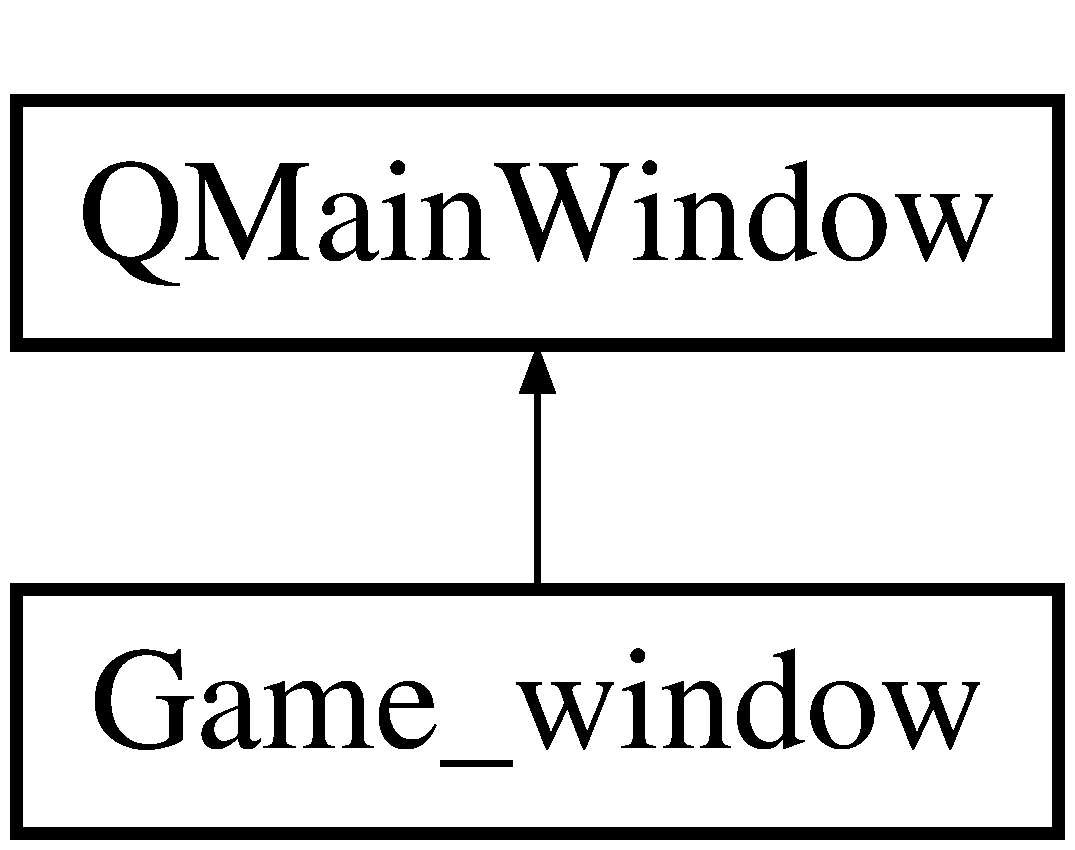
\includegraphics[height=2.000000cm]{class_game__window}
\end{center}
\end{figure}
\subsection*{Public Member Functions}
\begin{DoxyCompactItemize}
\item 
\mbox{\hyperlink{class_game__window_a48f330b2a2d893f271a2a854e116b54c}{Game\+\_\+window}} (Q\+Widget $\ast$parent=0, Q\+Host\+Address \+\_\+address=Q\+Host\+Address(\char`\"{}0\char`\"{}), uint \+\_\+port=0)
\item 
\mbox{\hyperlink{class_game__window_a5e84f0f55c4526bb0ea3a592c439c16f}{$\sim$\+Game\+\_\+window}} ()
\end{DoxyCompactItemize}
\subsection*{Protected Member Functions}
\begin{DoxyCompactItemize}
\item 
\mbox{\Hypertarget{class_game__window_a26801612466cd18f629107ed596bb0f1}\label{class_game__window_a26801612466cd18f629107ed596bb0f1}} 
void {\bfseries key\+Press\+Event} (Q\+Key\+Event $\ast$event)
\end{DoxyCompactItemize}


\subsection{Constructor \& Destructor Documentation}
\mbox{\Hypertarget{class_game__window_a48f330b2a2d893f271a2a854e116b54c}\label{class_game__window_a48f330b2a2d893f271a2a854e116b54c}} 
\index{Game\+\_\+window@{Game\+\_\+window}!Game\+\_\+window@{Game\+\_\+window}}
\index{Game\+\_\+window@{Game\+\_\+window}!Game\+\_\+window@{Game\+\_\+window}}
\subsubsection{\texorpdfstring{Game\+\_\+window()}{Game\_window()}}
{\footnotesize\ttfamily Game\+\_\+window\+::\+Game\+\_\+window (\begin{DoxyParamCaption}\item[{Q\+Widget $\ast$}]{parent = {\ttfamily 0},  }\item[{Q\+Host\+Address}]{\+\_\+address = {\ttfamily QHostAddress(\char`\"{}0\char`\"{})},  }\item[{uint}]{\+\_\+port = {\ttfamily 0} }\end{DoxyParamCaption})\hspace{0.3cm}{\ttfamily [explicit]}}

Initialize member variables, create game window and scene, populate the scene, connect to server and prepare game to start \mbox{\Hypertarget{class_game__window_a5e84f0f55c4526bb0ea3a592c439c16f}\label{class_game__window_a5e84f0f55c4526bb0ea3a592c439c16f}} 
\index{Game\+\_\+window@{Game\+\_\+window}!````~Game\+\_\+window@{$\sim$\+Game\+\_\+window}}
\index{````~Game\+\_\+window@{$\sim$\+Game\+\_\+window}!Game\+\_\+window@{Game\+\_\+window}}
\subsubsection{\texorpdfstring{$\sim$\+Game\+\_\+window()}{~Game\_window()}}
{\footnotesize\ttfamily Game\+\_\+window\+::$\sim$\+Game\+\_\+window (\begin{DoxyParamCaption}{ }\end{DoxyParamCaption})}

Delete dynamically allocated objects 

The documentation for this class was generated from the following files\+:\begin{DoxyCompactItemize}
\item 
C\+:/\+Users/\+Adam/\+Documents/\+Pacman\+\_\+\+Multiplayer-\/-\/-\/\+Client-\/\+App/Game\+\_\+window.\+h\item 
C\+:/\+Users/\+Adam/\+Documents/\+Pacman\+\_\+\+Multiplayer-\/-\/-\/\+Client-\/\+App/Game\+\_\+window.\+cpp\end{DoxyCompactItemize}

\hypertarget{class_ghost}{}\section{Ghost Class Reference}
\label{class_ghost}\index{Ghost@{Ghost}}
\subsection*{Public Member Functions}
\begin{DoxyCompactItemize}
\item 
\mbox{\hyperlink{class_ghost_a2e38d3c0c8546cceb74777b49a8e3bb7}{Ghost}} ()
\item 
void \mbox{\hyperlink{class_ghost_a51900002936b06acc029c845d9cb9240}{Reset}} ()
\item 
void \mbox{\hyperlink{class_ghost_a1f3b792655f805a40ebadd5651d0aa2a}{set\+Ghost\+\_\+X}} (int x)
\item 
void \mbox{\hyperlink{class_ghost_add5ef21063781debb4568305fd765162}{set\+Ghost\+\_\+Y}} (int y)
\item 
void \mbox{\hyperlink{class_ghost_a6e6f3e5ff87c2c9efeb58c188530f431}{set\+Is\+Scared}} (bool option)
\item 
void \mbox{\hyperlink{class_ghost_a22197187d8c42a2a2d2f0facdda54356}{set\+Scared\+White}} (bool option)
\item 
void \mbox{\hyperlink{class_ghost_a021a76713a5fdf501fd601d8644002bb}{set\+Ghost\+Direction}} (int dir)
\item 
void \mbox{\hyperlink{class_ghost_a3db876d86c02629c3a1aca84f63d4b70}{set\+Next\+Ghost\+Direction}} (int dir)
\item 
void \mbox{\hyperlink{class_ghost_ac57d9cbbba11f9c1b2bad35de42b417a}{set\+Scarestate}} (int \+\_\+scarestate)
\item 
void \mbox{\hyperlink{class_ghost_a0fa6a3ef0c3f9e33f6271fb5d2db2e24}{increment\+Scarestate}} ()
\item 
int \mbox{\hyperlink{class_ghost_aedf007ec72dec676c77734d29eedb2a8}{get\+Ghost\+\_\+X}} () const
\item 
int \mbox{\hyperlink{class_ghost_ae069b2ac96e5d13b5bd62cb1e75acf05}{get\+Ghost\+\_\+Y}} () const
\item 
int \mbox{\hyperlink{class_ghost_a3e8e504b59439d1fac4a72c2f55839c4}{get\+Ghost\+Direction}} () const
\item 
int \mbox{\hyperlink{class_ghost_a79c2a1a910758ead53489ab220c0bb3a}{get\+Next\+Ghost\+Direction}} () const
\item 
int \mbox{\hyperlink{class_ghost_a569122ead6a222f16e5603698b6b45e2}{get\+Scarestate}} () const
\item 
bool \mbox{\hyperlink{class_ghost_a36454848ec5fc01511d6d0a2ab81e21b}{get\+Is\+Scared}} () const
\item 
bool \mbox{\hyperlink{class_ghost_a052109c06bca7263f6bd0ccc963d5c48}{get\+Scared\+White}} () const
\end{DoxyCompactItemize}


\subsection{Constructor \& Destructor Documentation}
\mbox{\Hypertarget{class_ghost_a2e38d3c0c8546cceb74777b49a8e3bb7}\label{class_ghost_a2e38d3c0c8546cceb74777b49a8e3bb7}} 
\index{Ghost@{Ghost}!Ghost@{Ghost}}
\index{Ghost@{Ghost}!Ghost@{Ghost}}
\subsubsection{\texorpdfstring{Ghost()}{Ghost()}}
{\footnotesize\ttfamily Ghost\+::\+Ghost (\begin{DoxyParamCaption}{ }\end{DoxyParamCaption})}

Initialize ghost position and direction of movement 

\subsection{Member Function Documentation}
\mbox{\Hypertarget{class_ghost_aedf007ec72dec676c77734d29eedb2a8}\label{class_ghost_aedf007ec72dec676c77734d29eedb2a8}} 
\index{Ghost@{Ghost}!get\+Ghost\+\_\+X@{get\+Ghost\+\_\+X}}
\index{get\+Ghost\+\_\+X@{get\+Ghost\+\_\+X}!Ghost@{Ghost}}
\subsubsection{\texorpdfstring{get\+Ghost\+\_\+\+X()}{getGhost\_X()}}
{\footnotesize\ttfamily int Ghost\+::get\+Ghost\+\_\+X (\begin{DoxyParamCaption}{ }\end{DoxyParamCaption}) const\hspace{0.3cm}{\ttfamily [inline]}}

Get ghost x coordinate in form of int \mbox{\Hypertarget{class_ghost_ae069b2ac96e5d13b5bd62cb1e75acf05}\label{class_ghost_ae069b2ac96e5d13b5bd62cb1e75acf05}} 
\index{Ghost@{Ghost}!get\+Ghost\+\_\+Y@{get\+Ghost\+\_\+Y}}
\index{get\+Ghost\+\_\+Y@{get\+Ghost\+\_\+Y}!Ghost@{Ghost}}
\subsubsection{\texorpdfstring{get\+Ghost\+\_\+\+Y()}{getGhost\_Y()}}
{\footnotesize\ttfamily int Ghost\+::get\+Ghost\+\_\+Y (\begin{DoxyParamCaption}{ }\end{DoxyParamCaption}) const\hspace{0.3cm}{\ttfamily [inline]}}

Get ghost y coordinate in form of int \mbox{\Hypertarget{class_ghost_a3e8e504b59439d1fac4a72c2f55839c4}\label{class_ghost_a3e8e504b59439d1fac4a72c2f55839c4}} 
\index{Ghost@{Ghost}!get\+Ghost\+Direction@{get\+Ghost\+Direction}}
\index{get\+Ghost\+Direction@{get\+Ghost\+Direction}!Ghost@{Ghost}}
\subsubsection{\texorpdfstring{get\+Ghost\+Direction()}{getGhostDirection()}}
{\footnotesize\ttfamily int Ghost\+::get\+Ghost\+Direction (\begin{DoxyParamCaption}{ }\end{DoxyParamCaption}) const\hspace{0.3cm}{\ttfamily [inline]}}

Get ghost direction of movement in form of int \mbox{\Hypertarget{class_ghost_a36454848ec5fc01511d6d0a2ab81e21b}\label{class_ghost_a36454848ec5fc01511d6d0a2ab81e21b}} 
\index{Ghost@{Ghost}!get\+Is\+Scared@{get\+Is\+Scared}}
\index{get\+Is\+Scared@{get\+Is\+Scared}!Ghost@{Ghost}}
\subsubsection{\texorpdfstring{get\+Is\+Scared()}{getIsScared()}}
{\footnotesize\ttfamily bool Ghost\+::get\+Is\+Scared (\begin{DoxyParamCaption}{ }\end{DoxyParamCaption}) const\hspace{0.3cm}{\ttfamily [inline]}}

Check if ghost is scared blue and return bool \mbox{\Hypertarget{class_ghost_a79c2a1a910758ead53489ab220c0bb3a}\label{class_ghost_a79c2a1a910758ead53489ab220c0bb3a}} 
\index{Ghost@{Ghost}!get\+Next\+Ghost\+Direction@{get\+Next\+Ghost\+Direction}}
\index{get\+Next\+Ghost\+Direction@{get\+Next\+Ghost\+Direction}!Ghost@{Ghost}}
\subsubsection{\texorpdfstring{get\+Next\+Ghost\+Direction()}{getNextGhostDirection()}}
{\footnotesize\ttfamily int Ghost\+::get\+Next\+Ghost\+Direction (\begin{DoxyParamCaption}{ }\end{DoxyParamCaption}) const\hspace{0.3cm}{\ttfamily [inline]}}

Get next ghost direction of movement in form of int \mbox{\Hypertarget{class_ghost_a052109c06bca7263f6bd0ccc963d5c48}\label{class_ghost_a052109c06bca7263f6bd0ccc963d5c48}} 
\index{Ghost@{Ghost}!get\+Scared\+White@{get\+Scared\+White}}
\index{get\+Scared\+White@{get\+Scared\+White}!Ghost@{Ghost}}
\subsubsection{\texorpdfstring{get\+Scared\+White()}{getScaredWhite()}}
{\footnotesize\ttfamily bool Ghost\+::get\+Scared\+White (\begin{DoxyParamCaption}{ }\end{DoxyParamCaption}) const\hspace{0.3cm}{\ttfamily [inline]}}

Check if ghost is scared white and return bool \mbox{\Hypertarget{class_ghost_a569122ead6a222f16e5603698b6b45e2}\label{class_ghost_a569122ead6a222f16e5603698b6b45e2}} 
\index{Ghost@{Ghost}!get\+Scarestate@{get\+Scarestate}}
\index{get\+Scarestate@{get\+Scarestate}!Ghost@{Ghost}}
\subsubsection{\texorpdfstring{get\+Scarestate()}{getScarestate()}}
{\footnotesize\ttfamily int Ghost\+::get\+Scarestate (\begin{DoxyParamCaption}{ }\end{DoxyParamCaption}) const\hspace{0.3cm}{\ttfamily [inline]}}

Get ghost scarestate in form of int \mbox{\Hypertarget{class_ghost_a0fa6a3ef0c3f9e33f6271fb5d2db2e24}\label{class_ghost_a0fa6a3ef0c3f9e33f6271fb5d2db2e24}} 
\index{Ghost@{Ghost}!increment\+Scarestate@{increment\+Scarestate}}
\index{increment\+Scarestate@{increment\+Scarestate}!Ghost@{Ghost}}
\subsubsection{\texorpdfstring{increment\+Scarestate()}{incrementScarestate()}}
{\footnotesize\ttfamily void Ghost\+::increment\+Scarestate (\begin{DoxyParamCaption}{ }\end{DoxyParamCaption})\hspace{0.3cm}{\ttfamily [inline]}}

Increment ghost scarestate \mbox{\Hypertarget{class_ghost_a51900002936b06acc029c845d9cb9240}\label{class_ghost_a51900002936b06acc029c845d9cb9240}} 
\index{Ghost@{Ghost}!Reset@{Reset}}
\index{Reset@{Reset}!Ghost@{Ghost}}
\subsubsection{\texorpdfstring{Reset()}{Reset()}}
{\footnotesize\ttfamily void Ghost\+::\+Reset (\begin{DoxyParamCaption}{ }\end{DoxyParamCaption})}

Reset ghost position and direction of movement \mbox{\Hypertarget{class_ghost_a1f3b792655f805a40ebadd5651d0aa2a}\label{class_ghost_a1f3b792655f805a40ebadd5651d0aa2a}} 
\index{Ghost@{Ghost}!set\+Ghost\+\_\+X@{set\+Ghost\+\_\+X}}
\index{set\+Ghost\+\_\+X@{set\+Ghost\+\_\+X}!Ghost@{Ghost}}
\subsubsection{\texorpdfstring{set\+Ghost\+\_\+\+X()}{setGhost\_X()}}
{\footnotesize\ttfamily void Ghost\+::set\+Ghost\+\_\+X (\begin{DoxyParamCaption}\item[{int}]{x }\end{DoxyParamCaption})\hspace{0.3cm}{\ttfamily [inline]}}

Set ghost x coordinate \mbox{\Hypertarget{class_ghost_add5ef21063781debb4568305fd765162}\label{class_ghost_add5ef21063781debb4568305fd765162}} 
\index{Ghost@{Ghost}!set\+Ghost\+\_\+Y@{set\+Ghost\+\_\+Y}}
\index{set\+Ghost\+\_\+Y@{set\+Ghost\+\_\+Y}!Ghost@{Ghost}}
\subsubsection{\texorpdfstring{set\+Ghost\+\_\+\+Y()}{setGhost\_Y()}}
{\footnotesize\ttfamily void Ghost\+::set\+Ghost\+\_\+Y (\begin{DoxyParamCaption}\item[{int}]{y }\end{DoxyParamCaption})\hspace{0.3cm}{\ttfamily [inline]}}

Set ghost y coordinate \mbox{\Hypertarget{class_ghost_a021a76713a5fdf501fd601d8644002bb}\label{class_ghost_a021a76713a5fdf501fd601d8644002bb}} 
\index{Ghost@{Ghost}!set\+Ghost\+Direction@{set\+Ghost\+Direction}}
\index{set\+Ghost\+Direction@{set\+Ghost\+Direction}!Ghost@{Ghost}}
\subsubsection{\texorpdfstring{set\+Ghost\+Direction()}{setGhostDirection()}}
{\footnotesize\ttfamily void Ghost\+::set\+Ghost\+Direction (\begin{DoxyParamCaption}\item[{int}]{dir }\end{DoxyParamCaption})\hspace{0.3cm}{\ttfamily [inline]}}

Set ghost direction of movement \mbox{\Hypertarget{class_ghost_a6e6f3e5ff87c2c9efeb58c188530f431}\label{class_ghost_a6e6f3e5ff87c2c9efeb58c188530f431}} 
\index{Ghost@{Ghost}!set\+Is\+Scared@{set\+Is\+Scared}}
\index{set\+Is\+Scared@{set\+Is\+Scared}!Ghost@{Ghost}}
\subsubsection{\texorpdfstring{set\+Is\+Scared()}{setIsScared()}}
{\footnotesize\ttfamily void Ghost\+::set\+Is\+Scared (\begin{DoxyParamCaption}\item[{bool}]{option }\end{DoxyParamCaption})\hspace{0.3cm}{\ttfamily [inline]}}

Set if ghost is scared blue \mbox{\Hypertarget{class_ghost_a3db876d86c02629c3a1aca84f63d4b70}\label{class_ghost_a3db876d86c02629c3a1aca84f63d4b70}} 
\index{Ghost@{Ghost}!set\+Next\+Ghost\+Direction@{set\+Next\+Ghost\+Direction}}
\index{set\+Next\+Ghost\+Direction@{set\+Next\+Ghost\+Direction}!Ghost@{Ghost}}
\subsubsection{\texorpdfstring{set\+Next\+Ghost\+Direction()}{setNextGhostDirection()}}
{\footnotesize\ttfamily void Ghost\+::set\+Next\+Ghost\+Direction (\begin{DoxyParamCaption}\item[{int}]{dir }\end{DoxyParamCaption})\hspace{0.3cm}{\ttfamily [inline]}}

Set next ghost direction of movement \mbox{\Hypertarget{class_ghost_a22197187d8c42a2a2d2f0facdda54356}\label{class_ghost_a22197187d8c42a2a2d2f0facdda54356}} 
\index{Ghost@{Ghost}!set\+Scared\+White@{set\+Scared\+White}}
\index{set\+Scared\+White@{set\+Scared\+White}!Ghost@{Ghost}}
\subsubsection{\texorpdfstring{set\+Scared\+White()}{setScaredWhite()}}
{\footnotesize\ttfamily void Ghost\+::set\+Scared\+White (\begin{DoxyParamCaption}\item[{bool}]{option }\end{DoxyParamCaption})\hspace{0.3cm}{\ttfamily [inline]}}

Set if ghost is scared white \mbox{\Hypertarget{class_ghost_ac57d9cbbba11f9c1b2bad35de42b417a}\label{class_ghost_ac57d9cbbba11f9c1b2bad35de42b417a}} 
\index{Ghost@{Ghost}!set\+Scarestate@{set\+Scarestate}}
\index{set\+Scarestate@{set\+Scarestate}!Ghost@{Ghost}}
\subsubsection{\texorpdfstring{set\+Scarestate()}{setScarestate()}}
{\footnotesize\ttfamily void Ghost\+::set\+Scarestate (\begin{DoxyParamCaption}\item[{int}]{\+\_\+scarestate }\end{DoxyParamCaption})\hspace{0.3cm}{\ttfamily [inline]}}

Set ghost scarestate 

The documentation for this class was generated from the following files\+:\begin{DoxyCompactItemize}
\item 
C\+:/\+Users/\+Adam/\+Documents/\+Pacman\+\_\+\+Multiplayer-\/-\/-\/\+Server-\/\+App/ghost.\+h\item 
C\+:/\+Users/\+Adam/\+Documents/\+Pacman\+\_\+\+Multiplayer-\/-\/-\/\+Server-\/\+App/ghost.\+cpp\end{DoxyCompactItemize}

\hypertarget{class_map}{}\section{Map Class Reference}
\label{class_map}\index{Map@{Map}}
\subsection*{Public Member Functions}
\begin{DoxyCompactItemize}
\item 
\mbox{\hyperlink{class_map_a0f5ad0fd4563497b4214038cbca8b582}{Map}} ()
\item 
bool \mbox{\hyperlink{class_map_a1d4e431479ebaab122888188e12b912f}{Is\+Point\+Available}} (Q\+Point point)
\item 
Q\+Vector$<$ Q\+Point $>$ \mbox{\hyperlink{class_map_a461dfb2525afb9afbe88f1958c56ca04}{get\+Pacman\+Paths}} () const
\end{DoxyCompactItemize}


\subsection{Constructor \& Destructor Documentation}
\mbox{\Hypertarget{class_map_a0f5ad0fd4563497b4214038cbca8b582}\label{class_map_a0f5ad0fd4563497b4214038cbca8b582}} 
\index{Map@{Map}!Map@{Map}}
\index{Map@{Map}!Map@{Map}}
\subsubsection{\texorpdfstring{Map()}{Map()}}
{\footnotesize\ttfamily Map\+::\+Map (\begin{DoxyParamCaption}{ }\end{DoxyParamCaption})}

Create path points where movement is possible on map 

\subsection{Member Function Documentation}
\mbox{\Hypertarget{class_map_a461dfb2525afb9afbe88f1958c56ca04}\label{class_map_a461dfb2525afb9afbe88f1958c56ca04}} 
\index{Map@{Map}!get\+Pacman\+Paths@{get\+Pacman\+Paths}}
\index{get\+Pacman\+Paths@{get\+Pacman\+Paths}!Map@{Map}}
\subsubsection{\texorpdfstring{get\+Pacman\+Paths()}{getPacmanPaths()}}
{\footnotesize\ttfamily Q\+Vector$<$Q\+Point$>$ Map\+::get\+Pacman\+Paths (\begin{DoxyParamCaption}{ }\end{DoxyParamCaption}) const\hspace{0.3cm}{\ttfamily [inline]}}

Get pacman possible paths in form of Q\+Vector$<$\+Q\+Point$>$ \mbox{\Hypertarget{class_map_a1d4e431479ebaab122888188e12b912f}\label{class_map_a1d4e431479ebaab122888188e12b912f}} 
\index{Map@{Map}!Is\+Point\+Available@{Is\+Point\+Available}}
\index{Is\+Point\+Available@{Is\+Point\+Available}!Map@{Map}}
\subsubsection{\texorpdfstring{Is\+Point\+Available()}{IsPointAvailable()}}
{\footnotesize\ttfamily bool Map\+::\+Is\+Point\+Available (\begin{DoxyParamCaption}\item[{Q\+Point}]{point }\end{DoxyParamCaption})}

Check if point is present in map paths and return bool 

The documentation for this class was generated from the following files\+:\begin{DoxyCompactItemize}
\item 
C\+:/\+Users/\+Adam/\+Documents/\+Pacman\+\_\+\+Multiplayer-\/-\/-\/\+Server-\/\+App/map.\+h\item 
C\+:/\+Users/\+Adam/\+Documents/\+Pacman\+\_\+\+Multiplayer-\/-\/-\/\+Server-\/\+App/map.\+cpp\end{DoxyCompactItemize}

\hypertarget{class_pacman}{}\section{Pacman Class Reference}
\label{class_pacman}\index{Pacman@{Pacman}}
Inheritance diagram for Pacman\+:\begin{figure}[H]
\begin{center}
\leavevmode
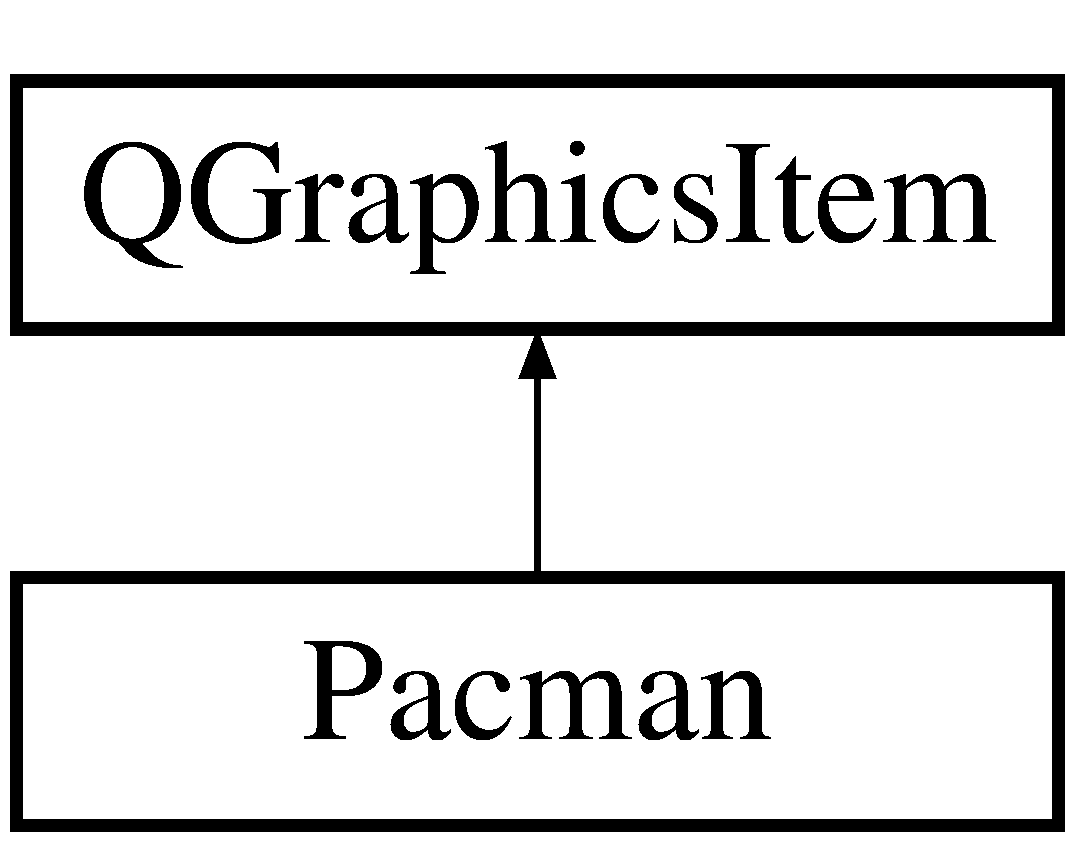
\includegraphics[height=2.000000cm]{class_pacman}
\end{center}
\end{figure}
\subsection*{Public Member Functions}
\begin{DoxyCompactItemize}
\item 
\mbox{\hyperlink{class_pacman_a499408baab38f119ebd4f41e90fbe3fe}{Pacman}} ()
\item 
void \mbox{\hyperlink{class_pacman_a560007dd011f202daaac68068c527e09}{advance}} ()
\item 
void \mbox{\hyperlink{class_pacman_a532e817b83bc0315b2ab666b2c90ab1a}{set\+Pac\+\_\+X}} (int)
\item 
void \mbox{\hyperlink{class_pacman_ad8250d3b6e8e9300bfe9ab650edca7e1}{set\+Pac\+\_\+Y}} (int)
\item 
void \mbox{\hyperlink{class_pacman_a388f4708c08ba930b471237a897f522e}{set\+Direction}} (int dir)
\end{DoxyCompactItemize}


\subsection{Constructor \& Destructor Documentation}
\mbox{\Hypertarget{class_pacman_a499408baab38f119ebd4f41e90fbe3fe}\label{class_pacman_a499408baab38f119ebd4f41e90fbe3fe}} 
\index{Pacman@{Pacman}!Pacman@{Pacman}}
\index{Pacman@{Pacman}!Pacman@{Pacman}}
\subsubsection{\texorpdfstring{Pacman()}{Pacman()}}
{\footnotesize\ttfamily Pacman\+::\+Pacman (\begin{DoxyParamCaption}{ }\end{DoxyParamCaption})}

Initialize member variables and load pacman images 

\subsection{Member Function Documentation}
\mbox{\Hypertarget{class_pacman_a560007dd011f202daaac68068c527e09}\label{class_pacman_a560007dd011f202daaac68068c527e09}} 
\index{Pacman@{Pacman}!advance@{advance}}
\index{advance@{advance}!Pacman@{Pacman}}
\subsubsection{\texorpdfstring{advance()}{advance()}}
{\footnotesize\ttfamily void Pacman\+::advance (\begin{DoxyParamCaption}{ }\end{DoxyParamCaption})}

Increment pacman\textquotesingle{}s animation state \mbox{\Hypertarget{class_pacman_a388f4708c08ba930b471237a897f522e}\label{class_pacman_a388f4708c08ba930b471237a897f522e}} 
\index{Pacman@{Pacman}!set\+Direction@{set\+Direction}}
\index{set\+Direction@{set\+Direction}!Pacman@{Pacman}}
\subsubsection{\texorpdfstring{set\+Direction()}{setDirection()}}
{\footnotesize\ttfamily void Pacman\+::set\+Direction (\begin{DoxyParamCaption}\item[{int}]{dir }\end{DoxyParamCaption})}

Set pacman direction of movement \mbox{\Hypertarget{class_pacman_a532e817b83bc0315b2ab666b2c90ab1a}\label{class_pacman_a532e817b83bc0315b2ab666b2c90ab1a}} 
\index{Pacman@{Pacman}!set\+Pac\+\_\+X@{set\+Pac\+\_\+X}}
\index{set\+Pac\+\_\+X@{set\+Pac\+\_\+X}!Pacman@{Pacman}}
\subsubsection{\texorpdfstring{set\+Pac\+\_\+\+X()}{setPac\_X()}}
{\footnotesize\ttfamily void Pacman\+::set\+Pac\+\_\+X (\begin{DoxyParamCaption}\item[{int}]{x }\end{DoxyParamCaption})}

Set pacman x coordinate \mbox{\Hypertarget{class_pacman_ad8250d3b6e8e9300bfe9ab650edca7e1}\label{class_pacman_ad8250d3b6e8e9300bfe9ab650edca7e1}} 
\index{Pacman@{Pacman}!set\+Pac\+\_\+Y@{set\+Pac\+\_\+Y}}
\index{set\+Pac\+\_\+Y@{set\+Pac\+\_\+Y}!Pacman@{Pacman}}
\subsubsection{\texorpdfstring{set\+Pac\+\_\+\+Y()}{setPac\_Y()}}
{\footnotesize\ttfamily void Pacman\+::set\+Pac\+\_\+Y (\begin{DoxyParamCaption}\item[{int}]{y }\end{DoxyParamCaption})}

Set pacman y coordinate 

The documentation for this class was generated from the following files\+:\begin{DoxyCompactItemize}
\item 
C\+:/\+Users/\+Adam/\+Documents/\+Pacman\+\_\+\+Multiplayer-\/-\/-\/\+Client-\/\+App/pacman.\+h\item 
C\+:/\+Users/\+Adam/\+Documents/\+Pacman\+\_\+\+Multiplayer-\/-\/-\/\+Client-\/\+App/pacman.\+cpp\end{DoxyCompactItemize}

\hypertarget{class_power_ball}{}\section{Power\+Ball Class Reference}
\label{class_power_ball}\index{Power\+Ball@{Power\+Ball}}
\subsection*{Public Member Functions}
\begin{DoxyCompactItemize}
\item 
\mbox{\hyperlink{class_power_ball_a302335590af74067ed44079a4b475760}{Power\+Ball}} ()
\item 
Q\+Vector$<$ Q\+Point $>$ \mbox{\hyperlink{class_power_ball_a47a928407c16b40cff53eaa96cbdb213}{get\+Power\+Ball\+Positions}} ()
\end{DoxyCompactItemize}


\subsection{Constructor \& Destructor Documentation}
\mbox{\Hypertarget{class_power_ball_a302335590af74067ed44079a4b475760}\label{class_power_ball_a302335590af74067ed44079a4b475760}} 
\index{Power\+Ball@{Power\+Ball}!Power\+Ball@{Power\+Ball}}
\index{Power\+Ball@{Power\+Ball}!Power\+Ball@{Power\+Ball}}
\subsubsection{\texorpdfstring{Power\+Ball()}{PowerBall()}}
{\footnotesize\ttfamily Power\+Ball\+::\+Power\+Ball (\begin{DoxyParamCaption}{ }\end{DoxyParamCaption})}

Fill powerballpositions vector with powerball positions represented as Q\+Points 

\subsection{Member Function Documentation}
\mbox{\Hypertarget{class_power_ball_a47a928407c16b40cff53eaa96cbdb213}\label{class_power_ball_a47a928407c16b40cff53eaa96cbdb213}} 
\index{Power\+Ball@{Power\+Ball}!get\+Power\+Ball\+Positions@{get\+Power\+Ball\+Positions}}
\index{get\+Power\+Ball\+Positions@{get\+Power\+Ball\+Positions}!Power\+Ball@{Power\+Ball}}
\subsubsection{\texorpdfstring{get\+Power\+Ball\+Positions()}{getPowerBallPositions()}}
{\footnotesize\ttfamily Q\+Vector$<$Q\+Point$>$ Power\+Ball\+::get\+Power\+Ball\+Positions (\begin{DoxyParamCaption}{ }\end{DoxyParamCaption})\hspace{0.3cm}{\ttfamily [inline]}}

Get powerball coordinates in form of Q\+Vector$<$\+Q\+Point$>$ 

The documentation for this class was generated from the following files\+:\begin{DoxyCompactItemize}
\item 
C\+:/\+Users/\+Adam/\+Documents/\+Pacman\+\_\+\+Multiplayer-\/-\/-\/\+Client-\/\+App/powerball.\+h\item 
C\+:/\+Users/\+Adam/\+Documents/\+Pacman\+\_\+\+Multiplayer-\/-\/-\/\+Client-\/\+App/powerball.\+cpp\end{DoxyCompactItemize}

\hypertarget{class_sounds}{}\section{Sounds Class Reference}
\label{class_sounds}\index{Sounds@{Sounds}}
\subsection*{Public Member Functions}
\begin{DoxyCompactItemize}
\item 
\mbox{\hyperlink{class_sounds_ab5cf288a278469c4d821a3ae33c39d37}{Sounds}} ()
\end{DoxyCompactItemize}
\subsection*{Public Attributes}
\begin{DoxyCompactItemize}
\item 
Q\+Media\+Player \mbox{\hyperlink{class_sounds_aa79b0142330a03976c36fe5c49a66c54}{beginning\+\_\+sound}}
\item 
Q\+Media\+Player \mbox{\hyperlink{class_sounds_a9821fc886ba3bfb8404bf9fee86ddfbe}{eat\+\_\+sound}}
\item 
Q\+Media\+Player \mbox{\hyperlink{class_sounds_a3c9fdf7f2d77cb9e9f4203e2e1a489f6}{eat\+\_\+ghost\+\_\+sound}}
\item 
Q\+Media\+Player \mbox{\hyperlink{class_sounds_a8c8a27c32ae161a18da0cc8c6df09e69}{pacman\+\_\+death\+\_\+sound}}
\end{DoxyCompactItemize}


\subsection{Constructor \& Destructor Documentation}
\mbox{\Hypertarget{class_sounds_ab5cf288a278469c4d821a3ae33c39d37}\label{class_sounds_ab5cf288a278469c4d821a3ae33c39d37}} 
\index{Sounds@{Sounds}!Sounds@{Sounds}}
\index{Sounds@{Sounds}!Sounds@{Sounds}}
\subsubsection{\texorpdfstring{Sounds()}{Sounds()}}
{\footnotesize\ttfamily Sounds\+::\+Sounds (\begin{DoxyParamCaption}{ }\end{DoxyParamCaption})}

Initialize sounds as Q\+Media\+Player objects binded to resource files containing proper sounds 

\subsection{Member Data Documentation}
\mbox{\Hypertarget{class_sounds_aa79b0142330a03976c36fe5c49a66c54}\label{class_sounds_aa79b0142330a03976c36fe5c49a66c54}} 
\index{Sounds@{Sounds}!beginning\+\_\+sound@{beginning\+\_\+sound}}
\index{beginning\+\_\+sound@{beginning\+\_\+sound}!Sounds@{Sounds}}
\subsubsection{\texorpdfstring{beginning\+\_\+sound}{beginning\_sound}}
{\footnotesize\ttfamily Q\+Media\+Player Sounds\+::beginning\+\_\+sound}

Sound played at beginning of game \mbox{\Hypertarget{class_sounds_a3c9fdf7f2d77cb9e9f4203e2e1a489f6}\label{class_sounds_a3c9fdf7f2d77cb9e9f4203e2e1a489f6}} 
\index{Sounds@{Sounds}!eat\+\_\+ghost\+\_\+sound@{eat\+\_\+ghost\+\_\+sound}}
\index{eat\+\_\+ghost\+\_\+sound@{eat\+\_\+ghost\+\_\+sound}!Sounds@{Sounds}}
\subsubsection{\texorpdfstring{eat\+\_\+ghost\+\_\+sound}{eat\_ghost\_sound}}
{\footnotesize\ttfamily Q\+Media\+Player Sounds\+::eat\+\_\+ghost\+\_\+sound}

Sound played when pacman eats ghost \mbox{\Hypertarget{class_sounds_a9821fc886ba3bfb8404bf9fee86ddfbe}\label{class_sounds_a9821fc886ba3bfb8404bf9fee86ddfbe}} 
\index{Sounds@{Sounds}!eat\+\_\+sound@{eat\+\_\+sound}}
\index{eat\+\_\+sound@{eat\+\_\+sound}!Sounds@{Sounds}}
\subsubsection{\texorpdfstring{eat\+\_\+sound}{eat\_sound}}
{\footnotesize\ttfamily Q\+Media\+Player Sounds\+::eat\+\_\+sound}

Sound played when foodball is eaten \mbox{\Hypertarget{class_sounds_a8c8a27c32ae161a18da0cc8c6df09e69}\label{class_sounds_a8c8a27c32ae161a18da0cc8c6df09e69}} 
\index{Sounds@{Sounds}!pacman\+\_\+death\+\_\+sound@{pacman\+\_\+death\+\_\+sound}}
\index{pacman\+\_\+death\+\_\+sound@{pacman\+\_\+death\+\_\+sound}!Sounds@{Sounds}}
\subsubsection{\texorpdfstring{pacman\+\_\+death\+\_\+sound}{pacman\_death\_sound}}
{\footnotesize\ttfamily Q\+Media\+Player Sounds\+::pacman\+\_\+death\+\_\+sound}

Sound played when pacman is eaten by ghost 

The documentation for this class was generated from the following files\+:\begin{DoxyCompactItemize}
\item 
C\+:/\+Users/\+Adam/\+Documents/\+Pacman\+\_\+\+Multiplayer-\/-\/-\/\+Client-\/\+App/sounds.\+h\item 
C\+:/\+Users/\+Adam/\+Documents/\+Pacman\+\_\+\+Multiplayer-\/-\/-\/\+Client-\/\+App/sounds.\+cpp\end{DoxyCompactItemize}

\hypertarget{class_text_screen_message}{}\section{Text\+Screen\+Message Class Reference}
\label{class_text_screen_message}\index{Text\+Screen\+Message@{Text\+Screen\+Message}}


{\ttfamily \#include $<$textscreenmessage.\+h$>$}

Inheritance diagram for Text\+Screen\+Message\+:\begin{figure}[H]
\begin{center}
\leavevmode
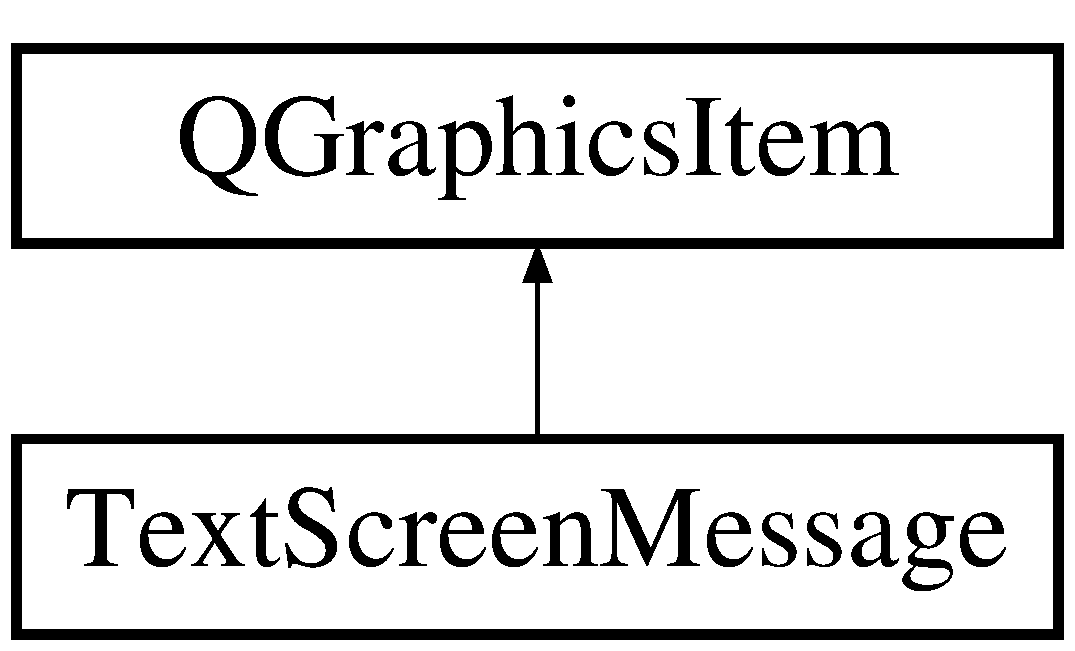
\includegraphics[height=2.000000cm]{class_text_screen_message}
\end{center}
\end{figure}
\subsection*{Public Member Functions}
\begin{DoxyCompactItemize}
\item 
\mbox{\hyperlink{class_text_screen_message_a662c1edab7a2fc1d87804fb54672d2dd}{Text\+Screen\+Message}} ()
\item 
void \mbox{\hyperlink{class_text_screen_message_aba833b25e9b57517d22d43560ceec249}{set\+Text\+State}} (Q\+String \+\_\+textstate)
\end{DoxyCompactItemize}


\subsection{Detailed Description}
Class responsible for displaying result of game 

\subsection{Constructor \& Destructor Documentation}
\mbox{\Hypertarget{class_text_screen_message_a662c1edab7a2fc1d87804fb54672d2dd}\label{class_text_screen_message_a662c1edab7a2fc1d87804fb54672d2dd}} 
\index{Text\+Screen\+Message@{Text\+Screen\+Message}!Text\+Screen\+Message@{Text\+Screen\+Message}}
\index{Text\+Screen\+Message@{Text\+Screen\+Message}!Text\+Screen\+Message@{Text\+Screen\+Message}}
\subsubsection{\texorpdfstring{Text\+Screen\+Message()}{TextScreenMessage()}}
{\footnotesize\ttfamily Text\+Screen\+Message\+::\+Text\+Screen\+Message (\begin{DoxyParamCaption}{ }\end{DoxyParamCaption})}

Initialize states of all member variables 

\subsection{Member Function Documentation}
\mbox{\Hypertarget{class_text_screen_message_aba833b25e9b57517d22d43560ceec249}\label{class_text_screen_message_aba833b25e9b57517d22d43560ceec249}} 
\index{Text\+Screen\+Message@{Text\+Screen\+Message}!set\+Text\+State@{set\+Text\+State}}
\index{set\+Text\+State@{set\+Text\+State}!Text\+Screen\+Message@{Text\+Screen\+Message}}
\subsubsection{\texorpdfstring{set\+Text\+State()}{setTextState()}}
{\footnotesize\ttfamily void Text\+Screen\+Message\+::set\+Text\+State (\begin{DoxyParamCaption}\item[{Q\+String}]{\+\_\+textstate }\end{DoxyParamCaption})}

Set what is supposed to be displayed by class 

The documentation for this class was generated from the following files\+:\begin{DoxyCompactItemize}
\item 
C\+:/\+Users/\+Adam/\+Documents/\+Pacman\+\_\+\+Multiplayer-\/-\/-\/\+Client-\/\+App/textscreenmessage.\+h\item 
C\+:/\+Users/\+Adam/\+Documents/\+Pacman\+\_\+\+Multiplayer-\/-\/-\/\+Client-\/\+App/textscreenmessage.\+cpp\end{DoxyCompactItemize}

%--- End generated contents ---

% Index
\backmatter
\newpage
\phantomsection
\clearemptydoublepage
\addcontentsline{toc}{chapter}{Index}
\printindex

\end{document}
